% =============================================================
% Methodology schematic for the CS495 capstone poster.
% Standalone preview:  pdflatex methodology_schematic.tex
% To embed in the poster: paste the \begin{tikzpicture}...\end{tikzpicture}
% block into the Methodology posterblock. The BC* colors are already defined
% in the poster preamble, so inside the poster you can delete the \definecolor
% lines below.
% =============================================================
\documentclass[border=12pt]{standalone}
\usepackage{tikz}
\usetikzlibrary{arrows.meta, positioning, fit, backgrounds}

% --- Bellevue College brand colors (already defined in the poster) ---
\definecolor{BCBlue}{HTML}{003D79}
\definecolor{BCSilver}{HTML}{A7A9AC}
\definecolor{BCRed}{HTML}{C4122F}
\definecolor{BCLightBlue}{HTML}{E6EEF7}
\definecolor{BCDarkBlue}{HTML}{002851}
\definecolor{BCInk}{HTML}{1A1A1A}

\begin{document}
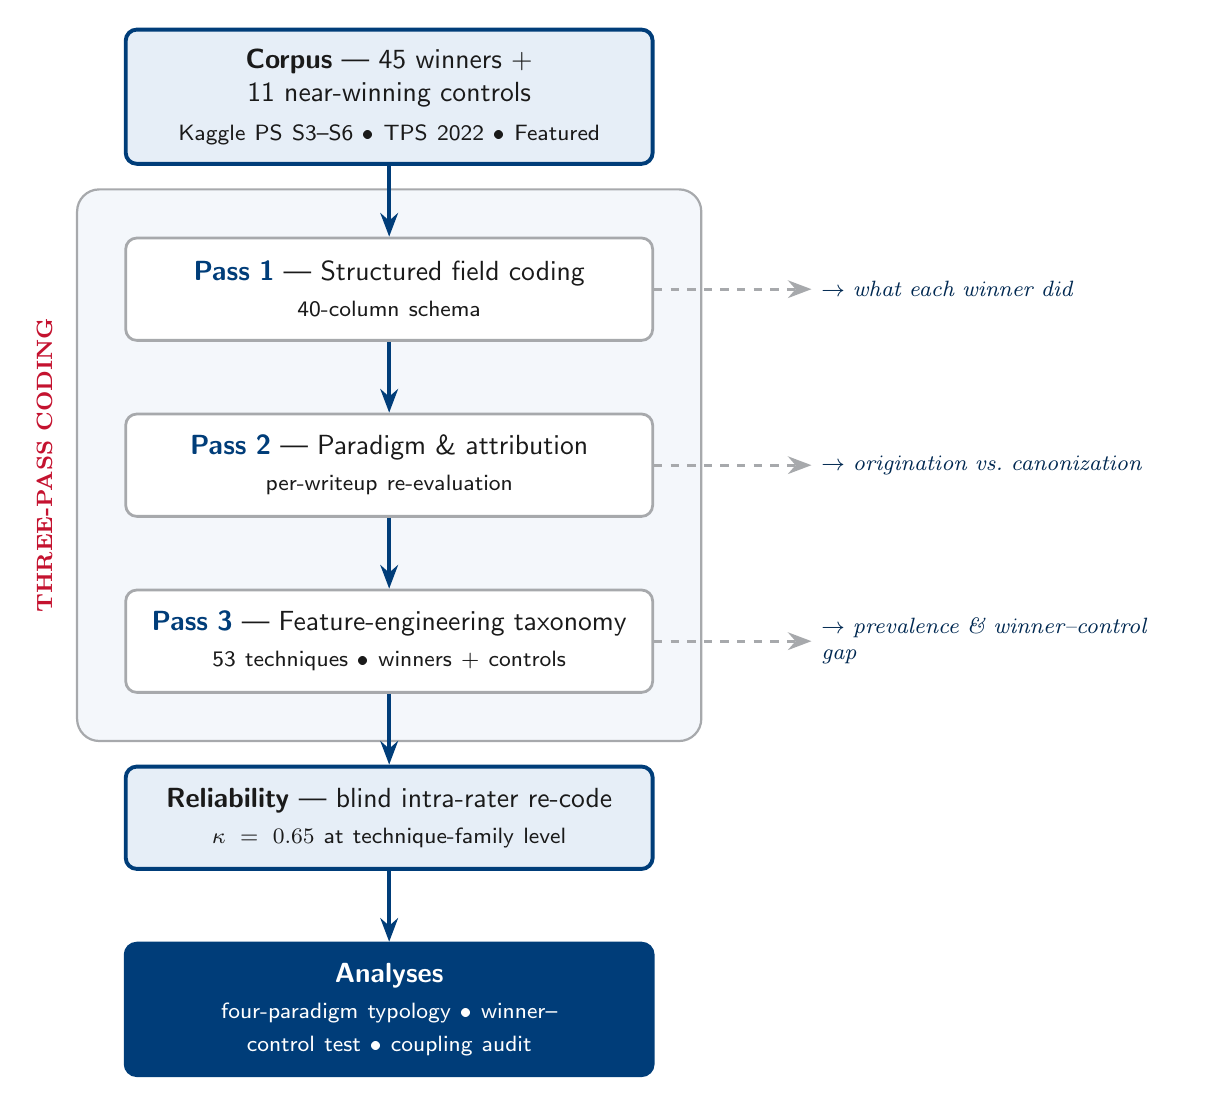
\begin{tikzpicture}[
  font=\sffamily,
  node distance=9mm,
  >={Stealth[length=3mm]},
  box/.style={rectangle, rounded corners=4pt, draw=BCSilver, line width=1pt,
              fill=white, text=BCInk, align=center, inner sep=7pt,
              minimum height=13mm, text width=62mm},
  source/.style={box, fill=BCLightBlue, draw=BCBlue, line width=1.4pt},
  rel/.style={box, fill=BCLightBlue, draw=BCBlue, line width=1.4pt},
  result/.style={box, fill=BCBlue, text=white, draw=BCBlue, line width=1.4pt},
  ann/.style={text=BCDarkBlue, font=\itshape\footnotesize, align=left, text width=46mm},
  arr/.style={->, draw=BCBlue, line width=1.3pt},
  yields/.style={->, draw=BCSilver, line width=1pt, dashed},
]

% --- spine ---
\node[source] (corpus)
  {\textbf{Corpus} --- 45 winners + 11 near-winning controls\\[2pt]
   \footnotesize Kaggle PS S3--S6 \textbullet\ TPS 2022 \textbullet\ Featured};

\node[box, below=of corpus] (p1)
  {\textbf{\textcolor{BCBlue}{Pass 1}} --- Structured field coding\\[1pt]
   \footnotesize 40-column schema};
\node[box, below=of p1] (p2)
  {\textbf{\textcolor{BCBlue}{Pass 2}} --- Paradigm \& attribution\\[1pt]
   \footnotesize per-writeup re-evaluation};
\node[box, below=of p2] (p3)
  {\textbf{\textcolor{BCBlue}{Pass 3}} --- Feature-engineering taxonomy\\[1pt]
   \footnotesize 53 techniques \textbullet\ winners + controls};

\node[rel, below=of p3] (reliab)
  {\textbf{Reliability} --- blind intra-rater re-code\\[1pt]
   \footnotesize $\kappa = 0.65$ at technique-family level};

\node[result, below=of reliab] (out)
  {\textbf{Analyses}\\[1pt]
   \footnotesize four-paradigm typology \textbullet\ winner--control test \textbullet\ coupling audit};

% --- per-pass "yields" annotations on the right ---
\node[ann, right=20mm of p1] (a1) {$\rightarrow$ what each winner did};
\node[ann, right=20mm of p2] (a2) {$\rightarrow$ origination vs.\ canonization};
\node[ann, right=20mm of p3] (a3) {$\rightarrow$ prevalence \& winner--control gap};

% --- spine arrows ---
\draw[arr] (corpus) -- (p1);
\draw[arr] (p1) -- (p2);
\draw[arr] (p2) -- (p3);
\draw[arr] (p3) -- (reliab);
\draw[arr] (reliab) -- (out);

% --- dashed connectors to annotations ---
\draw[yields] (p1.east) -- (a1.west);
\draw[yields] (p2.east) -- (a2.west);
\draw[yields] (p3.east) -- (a3.west);

% --- panel grouping the three passes ---
\begin{scope}[on background layer]
  \node[fill=BCLightBlue!45, rounded corners=8pt, draw=BCSilver, line width=0.8pt,
        fit=(p1)(p2)(p3), inner sep=6mm] (panel) {};
\end{scope}
\node[rotate=90, text=BCRed, font=\bfseries\footnotesize]
      at ([xshift=-4mm]panel.west) {THREE-PASS CODING};

\end{tikzpicture}
\end{document}
